% Created 2026-01-26 Mon 19:14
% Intended LaTeX compiler: pdflatex
\documentclass[presentation,aspectratio=1610]{beamer}
\usepackage[utf8]{inputenc}
\usepackage[T1]{fontenc}
\usepackage{graphicx}
\usepackage{longtable}
\usepackage{wrapfig}
\usepackage{rotating}
\usepackage[normalem]{ulem}
\usepackage{amsmath}
\usepackage{amssymb}
\usepackage{capt-of}
\usepackage{hyperref}
\setbeamertemplate{navigation symbols}{}
\setbeamertemplate{footline}[frame number]
\usepackage{pgfplots}
\usepgfplotslibrary{polar}
\pgfplotsset{compat=1.18}
\usepackage[height=3024]{beamer-reveal}
\usetheme{Madrid}
\usecolortheme{dolphin}
\usefonttheme{structurebold}
\author{Mohammad Durrani}
\date{\today}
\title{Course Overview and The Shell}
\subtitle{CMSC398W: Practical Tools For Efficient Development}
\hypersetup{
 pdfauthor={Mohammad Durrani},
 pdftitle={Course Overview and The Shell},
 pdfkeywords={},
 pdfsubject={},
 pdfcreator={Emacs 30.2 (Org mode 9.7.11)}, 
 pdflang={English}}
\begin{document}

\maketitle
\section*{About The Class}
\label{sec:org776c389}

\begin{frame}[label={sec:orgaccb531}]{About The Class}
\begin{block}{Course Information}
\alert{CMSC398W: Practical Tools For Efficient Development}

\begin{itemize}
\item Overview of tools used in development: command line, Git, debuggers, build systems, etc.
\item Emphasis on breadth over depth
\item Hands-on learning through projects
\end{itemize}
\end{block}
\begin{exampleblock}{Course Goals}\label{sec:org9b9bfe7}
\begin{itemize}
\item Improve your computing ecosystem literacy
\item Improve your efficiency
\item Reduce cognitive load while developing
\end{itemize}
\end{exampleblock}
\end{frame}
\begin{frame}[label={sec:orgf86fadb}]{About Me - Mohammad}
\begin{columns}
\begin{column}{0.55\columnwidth}
\alert{Mohammad Durrani}

\begin{itemize}
\item Senior
\item CS + Math, minor in Robotics
\item \alert{Previous Experience:}
\begin{itemize}
\item Teaching this class since Spring 2025
\item SWE Intern at Google in SF
\item SWE Intern at TRX Systems in Greenbelt
\end{itemize}
\end{itemize}
\end{column}
\begin{column}{0.4\columnwidth}
\alert{Hobbies:}

\begin{itemize}
\item Rock climbing
\item Basketball
\item Robots
\end{itemize}
\end{column}
\end{columns}
\end{frame}
\begin{frame}[label={sec:orgdea6ace}]{What To Expect}
\begin{block}{Course Structure}
\alert{Read the syllabus for all course related information!}
\end{block}
\begin{columns}
\begin{column}{0.48\columnwidth}
\begin{itemize}
\item Introduction of topic
\item Motivation / Real world example
\item Technical details
\end{itemize}
\end{column}
\begin{column}{0.48\columnwidth}
\begin{itemize}
\item Projects focusing on application
\item Best way to learn: \alert{use them}
\end{itemize}
\end{column}
\end{columns}
\end{frame}
\begin{frame}[label={sec:orgcaf83a8}]{Course Logistics}
\begin{alertblock}{Communication \& Submission}
\begin{itemize}
\item All course communication: \alert{Piazza}
\item All assignments submitted: \alert{Gradescope}
\item \alert{10\% per-day late penalty} (except the last project)
\end{itemize}
\end{alertblock}
\begin{block}{Grade Breakdown}
\begin{center}
\begin{tabular}{lll}
Percentage & Title & Description\\
\hline
80\% & Projects (20\% per) & 4 Major Projects\\
15\% & Application Days (5\% per) & Completion of Application Days\\
5\% & Participation & Participation in class\\
\end{tabular}
\end{center}
\end{block}
\end{frame}
\begin{frame}[label={sec:org4637796}]{Application Days}
\begin{block}{Based on Feedback}
Based on feedback from the previous iteration, we'll have days focused on using the tools we learn in class on toy problems.
\end{block}
\begin{exampleblock}<2->{Three Application Days}\label{sec:orgfadf8d0}
\begin{enumerate}
\item \alert{Shell}
\item \alert{Git}
\item \alert{Networking}
\end{enumerate}

\vspace{0.3em}
(Subject to change)
\end{exampleblock}
\end{frame}
\begin{frame}[label={sec:orgca362a2}]{Grade Distribution}
\begin{center}
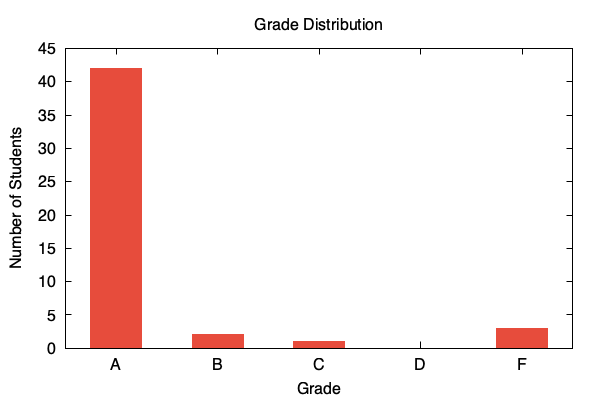
\includegraphics[width=.9\linewidth]{grade-pie.png}
\label{org5662816}
\end{center}
\end{frame}
\section*{The Shell}
\label{sec:orgceb7402}

\begin{frame}[label={sec:orgb8d8f7d}]{Introduction}
\begin{block}{Why The Shell?}
\begin{itemize}[<+->]
\item Traditional interfaces: graphical UIs, voice commands, AR/VR
\item Modern interfaces great for \textasciitilde{}80\% of use cases, but can be limiting
\item You cannot click a button that doesn't exist
\item You cannot give a voice command that hasn't been programmed
\item The shell provides a powerful \alert{text-based interface} with flexibility and control
\end{itemize}
\end{block}
\begin{exampleblock}<2->{Focus}\label{sec:orgcf01ddf}
\begin{itemize}
\item We'll focus on \alert{bash} (Bourne Again Shell)
\item One of the most widely used shells
\item Essential for developers, system administrators, and power users
\end{itemize}
\end{exampleblock}
\end{frame}
\begin{frame}[label={sec:org1126bdb}]{What is the Shell?}
\begin{definition}[Definition]\label{sec:orgb2e2f09}
\alert{Shell:} A program that allows you to execute commands and interface with your operating system.
\end{definition}
\begin{block}{Characteristics}
\begin{itemize}
\item Textual interface for computer interaction
\item Most platforms have a shell with many types (bash, zsh, dash, fish, etc.)
\item Requires a \alert{terminal} / \alert{terminal emulator} to interact with the shell
\item We will use \alert{bash} in this class (generally default on Linux)
\item macOS / Windows have different defaults
\end{itemize}
\end{block}
\begin{alertblock}<2->{Reference}
The \alert{Bash Reference Manual} contains everything you need to know about bash!
\end{alertblock}
\end{frame}
\begin{frame}[label={sec:org7bceb12}]{Important Terminology}
\begin{block}{1. Traditional Terminal}
\begin{itemize}
\item Historical computing device
\item Physical keyboard and screen connected to shared computer
\item Text-only interface (pre-mouse era)
\item Used specific protocols to communicate
\item Evolution: colors, different fonts, extended character sets
\end{itemize}
\end{block}
\begin{block}<2->{2. Modern Terminal Emulator}
Software that emulates traditional terminals

\alert{Examples by platform:}
\begin{itemize}
\item \alert{Windows:} CMD.exe, PowerShell, PuTTY, Windows Terminal
\item \alert{macOS:} Terminal.app, iTerm2
\item \alert{Linux:} xTerm, Gnome Terminal, Konsole, Kitty, Ghostty, Alacritty
\end{itemize}
\end{block}
\end{frame}
\begin{frame}[label={sec:org5829016}]{Terminal Emulator Features}
\begin{exampleblock}{Modern Features}\label{sec:org93dbe07}
\begin{itemize}
\item Supports tabs, split panes, and Unicode
\item Quality-of-life features:
\begin{itemize}
\item Search functionality
\item Copy/paste
\item Customizable appearance
\end{itemize}
\end{itemize}
\end{exampleblock}
\begin{definition}<2->[3. Shell/Command-line Interface]\label{sec:org010b5b9}
Program started when logging into terminal that interprets commands and provides interactive environment.
\end{definition}
\end{frame}
\begin{frame}[label={sec:orga5bf6f4}]{Motivation}
\begin{block}{Why Master the Command Line?}
\begin{itemize}[<+->]
\item \alert{Essential} for software development
\item Makes you \alert{much more efficient}
\item Many development tools are command line based
\item Access remote servers and cloud platforms
\item Automate repetitive tasks
\item Work across different operating systems
\end{itemize}
\end{block}
\end{frame}
\begin{frame}[label={sec:orge3a3f17},fragile]{The Prompt}
 \begin{block}{Anatomy of the Prompt}
\texttt{username@domain directory\$}
\end{block}
\begin{columns}
\begin{column}{1.0\columnwidth}
\begin{center}
\begin{tabular}{ll}
Component & Description\\
\hline
username & Currently logged in user\\
@ & Separator (convention)\\
domain & Machine name\\
directory & Current working directory\\
\$ & User-level shell indicator\\
\texttt{\#} & Root-level shell indicator\\
\end{tabular}
\end{center}
\end{column}
\end{columns}
\begin{alertblock}<2->{Note}
The prompt is customizable and can include additional information (git status, time, etc.)
\end{alertblock}
\end{frame}
\begin{frame}[label={sec:org51472af},fragile]{Basic Commands}
 \begin{block}{How Commands Work}
Inside a prompt you type a command, which is then executed or interpreted.

The shell:
\begin{enumerate}
\item Parses by splitting on whitespace
\item Runs the program indicated by the first word
\item Gives each subsequent word as an argument to the program
\end{enumerate}
\end{block}
\begin{alertblock}{Important Notes}
\begin{itemize}
\item Commands are \alert{case-sensitive}
\item Each command is a separate program (usually)
\item Arguments modify command behavior
\item Special characters need proper handling
\item Commands can accept flags/options starting with \texttt{-}
\end{itemize}
\end{alertblock}
\end{frame}
\begin{frame}[label={sec:org281b2e8},fragile]{Basic Commands - Examples}
 \begin{block}{Command Examples}
\begin{verbatim}
# Show current date and time
date

# Echo text to screen
echo hello

# Handle spaces in arguments
echo "Hello World"
echo Hello\ World

# Multiple arguments
echo first second third
\end{verbatim}
\end{block}
\end{frame}
\begin{frame}[label={sec:orgb1b9c68}]{PATH Variable}
\begin{definition}[What is PATH?]\label{sec:org9610dd6}
PATH is an environment variable that lists which directories the shell should search for programs.
\end{definition}
\begin{block}{Characteristics}
\begin{itemize}
\item Colon-separated list of directories
\item Shell searches directories in order
\item First matching executable is used
\item Can be modified to add new directories
\item Built-in commands take precedence over PATH
\end{itemize}
\end{block}
\end{frame}
\begin{frame}[label={sec:orgb43950d},fragile]{PATH Variable - Example}
 \begin{block}{Exploring PATH}
\begin{verbatim}
# Display PATH
cmsc398w:~$ echo $PATH
/usr/local/sbin:/usr/local/bin:/usr/sbin:
/usr/bin:/sbin:/bin:/snap/bin

# Find location of command
cmsc398w:~$ which echo
/usr/bin/echo

# Run directly without PATH
cmsc398w:~$ /bin/echo $PATH
/usr/local/sbin:/usr/local/bin:/usr/sbin:
/usr/bin:/sbin:/bin:/snap/bin
\end{verbatim}
\end{block}
\end{frame}
\begin{frame}[label={sec:org1f7491d},fragile]{Modifying PATH}
 \begin{exampleblock}{Adding to PATH}\label{sec:org27b42af}
\begin{verbatim}
export PATH="/Directory1:$PATH"
\end{verbatim}

This adds \texttt{/Directory1} to the beginning of your PATH, giving it priority in command searches.
\end{exampleblock}
\end{frame}
\begin{frame}[label={sec:org9128ee8},fragile]{Navigating - Paths}
 \begin{columns}
\begin{column}{0.48\columnwidth}
\begin{exampleblock}{}\label{sec:org9f7b308}
\begin{itemize}
\item Start with \texttt{/} (Unix) or drive letter (Windows)
\item Full path from root
\item Work from any location
\item \alert{Example:} \texttt{/home/user/docs}
\end{itemize}
\end{exampleblock}
\end{column}
\begin{column}{0.48\columnwidth}
\begin{exampleblock}{}\label{sec:org5f4ef1f}
\begin{itemize}
\item Relative to current directory
\item More concise
\item Context-dependent
\end{itemize}
\end{exampleblock}
\end{column}
\end{columns}
\begin{alertblock}{Special Directories}
\begin{center}
\begin{tabular}{ll}
Symbol & Meaning\\
\hline
\texttt{.} & Current directory\\
\texttt{..} & Parent directory\\
\texttt{\textasciitilde{}} & Home directory\\
\end{tabular}
\end{center}
\end{alertblock}
\end{frame}
\begin{frame}[label={sec:org325561b},fragile]{Essential Navigation Commands}
 \begin{block}{Commands}
\begin{center}
\begin{tabular}{ll}
Command & Description\\
\hline
\texttt{pwd} & Print working directory\\
\texttt{cd} & Change directory\\
\texttt{ls} & List directory contents\\
\texttt{ls -l} & Long format listing\\
\texttt{ls -a} & Show hidden files\\
\texttt{ls -lh} & Human-readable sizes\\
\end{tabular}
\end{center}
\end{block}
\end{frame}
\begin{frame}[label={sec:orgc580ee1},fragile]{Navigation Examples}
 \begin{block}{Using Navigation Commands}
\begin{verbatim}
# Show current directory
pwd

# Go to home directory
cd ~
cd

# Go to parent directory
cd ..

# Go to specific directory
cd /usr/local/bin

# Go to previous directory
cd -
\end{verbatim}
\end{block}
\end{frame}
\begin{frame}[label={sec:orgc2e74e6},fragile]{File and Directory Manipulation}
 \begin{block}{Common Operations}
\begin{center}
\begin{tabular}{ll}
Command & Description\\
\hline
\texttt{mkdir} & Make directory\\
\texttt{touch} & Create empty file / update timestamp\\
\texttt{cp} & Copy files/directories\\
\texttt{mv} & Move/rename files\\
\texttt{rm} & Remove files\\
\texttt{rmdir} & Remove empty directory\\
\end{tabular}
\end{center}
\end{block}
\begin{alertblock}<2->{Important Flags}
\begin{itemize}
\item \texttt{-r}: Recursive (for directories)
\item \texttt{-i}: Interactive (ask before overwrite)
\item \texttt{-f}: Force (no prompts)
\item \texttt{-v}: Verbose (show what's happening)
\end{itemize}
\end{alertblock}
\end{frame}
\begin{frame}[label={sec:org6359184},fragile]{File Manipulation Examples}
 \begin{block}{Examples}
\begin{verbatim}
# Create directory
mkdir new_folder
mkdir -p parent/child/grandchild

# Copy files
cp file.txt backup.txt
cp -r folder1 folder2

# Move/rename
mv old_name.txt new_name.txt
mv file.txt /path/to/destination/

# Remove files
rm file.txt
rm -r folder
rm -rf folder  # Force remove (careful!)
\end{verbatim}
\end{block}
\end{frame}
\begin{frame}[label={sec:org0a8ea09},fragile]{Viewing File Contents}
 \begin{block}{Viewing Commands}
\begin{center}
\begin{tabular}{ll}
Command & Description\\
\hline
\texttt{cat} & Display entire file\\
\texttt{less} & Page through file (q to quit)\\
\texttt{head} & Show first 10 lines\\
\texttt{tail} & Show last 10 lines\\
\texttt{tail -f} & Follow file updates (logs)\\
\end{tabular}
\end{center}
\end{block}
\end{frame}
\begin{frame}[label={sec:org446b267},fragile]{Viewing Examples}
 \begin{block}{File Viewing}
\begin{verbatim}
# Display entire file
cat file.txt

# Page through file
less file.txt

# First 20 lines
head -n 20 file.txt

# Last 15 lines
tail -n 15 file.txt

# Follow log file
tail -f /var/log/system.log
\end{verbatim}
\end{block}
\end{frame}
\begin{frame}[label={sec:orgba753ca},fragile]{Environment Variables}
 \begin{definition}[What are Environment Variables?]\label{sec:org53a65ff}
Variables that affect how processes run and are accessible to all child processes.
\end{definition}
\begin{block}{Common Variables}
\begin{center}
\begin{tabular}{ll}
Variable & Description\\
\hline
\texttt{PATH} & Command search path\\
\texttt{HOME} & User's home directory\\
\texttt{USER} & Current username\\
\texttt{SHELL} & Current shell\\
\texttt{PWD} & Current directory\\
\end{tabular}
\end{center}
\end{block}
\end{frame}
\begin{frame}[label={sec:orgbb0ff49},fragile]{Environment Variable Examples}
 \begin{block}{Working with Variables}
\begin{verbatim}
# Display variable
echo $PATH
echo $HOME

# Set variable (current session)
MY_VAR="value"
echo $MY_VAR

# Export variable (to child processes)
export MY_VAR="value"

# View all environment variables
env
printenv
\end{verbatim}
\end{block}
\end{frame}
\section*{Shell Tools}
\label{sec:orgdc9ee6a}

\begin{frame}[label={sec:orgb60a2c1},fragile]{Searching and Finding}
 \begin{block}{Search Commands}
\begin{center}
\begin{tabular}{ll}
Command & Description\\
\hline
\texttt{find} & Find files by name/type/size\\
\texttt{grep} & Search file contents\\
\texttt{which} & Locate command\\
\texttt{locate} & Fast file search (uses database)\\
\end{tabular}
\end{center}
\end{block}
\end{frame}
\begin{frame}[label={sec:orgaa91e2a},fragile]{Search Examples}
 \begin{block}{Finding Files and Content}
\begin{verbatim}
# Find files by name
find . -name "*.txt"
find /home -name "config.json"

# Find directories
find . -type d -name "test*"

# Search file contents
grep "error" logfile.txt
grep -r "TODO" .  # Recursive search
grep -i "warning" file.txt  # Case-insensitive

# Locate command
which python
\end{verbatim}
\end{block}
\end{frame}
\begin{frame}[label={sec:orgcfbf65a},fragile]{Advanced grep}
 \begin{block}{grep Options}
\begin{center}
\begin{tabular}{ll}
Option & Description\\
\hline
\texttt{-i} & Case-insensitive search\\
\texttt{-r} & Recursive search\\
\texttt{-v} & Invert match (show non-matching)\\
\texttt{-n} & Show line numbers\\
\texttt{-c} & Count matching lines\\
\texttt{-l} & Show only filenames\\
\texttt{-A N} & Show N lines after match\\
\texttt{-B N} & Show N lines before match\\
\texttt{-C N} & Show N lines before and after\\
\end{tabular}
\end{center}
\end{block}
\end{frame}
\begin{frame}[label={sec:org695b0e5},fragile]{grep Examples}
 \begin{block}{Advanced grep Usage}
\begin{verbatim}
# Find all TODO comments with context
grep -n -C 2 "TODO" *.py

# Count errors in log
grep -c "ERROR" application.log

# Find files containing pattern
grep -rl "import numpy" .

# Complex pattern matching
grep -E "error|warning|critical" logfile.txt

# Exclude pattern
grep -v "DEBUG" logfile.txt | less
\end{verbatim}
\end{block}
\end{frame}
\begin{frame}[label={sec:org9d1c15a},fragile]{Wildcards and Globbing}
 \begin{block}{Glob Patterns}
\begin{center}
\begin{tabular}{ll}
Pattern & Matches\\
\hline
\texttt{*} & Any string (including empty)\\
\texttt{?} & Any single character\\
\texttt{[abc]} & Any character in brackets\\
\texttt{[a-z]} & Any character in range\\
\texttt{[!abc]} & Any character NOT in brackets\\
\end{tabular}
\end{center}
\end{block}
\end{frame}
\begin{frame}[label={sec:org7b39188},fragile]{Globbing Examples}
 \begin{block}{Pattern Matching}
\begin{verbatim}
# All .txt files
ls *.txt

# Files starting with 'test'
ls test*

# Single character wildcard
ls file?.txt

# Character sets
ls file[123].txt
ls [a-z]*.txt

# Negation
ls [!a-z]*
\end{verbatim}
\end{block}
\end{frame}
\begin{frame}[label={sec:org84b8dbe},fragile]{Brace Expansion}
 \begin{definition}[Creating Multiple Arguments]\label{sec:org3ddc37b}
Brace expansion generates multiple strings from a pattern.
\end{definition}
\begin{block}{Examples}
\begin{verbatim}
# Create multiple files
touch file{1,2,3}.txt
# Creates: file1.txt, file2.txt, file3.txt

# Ranges
echo {1..10}
echo {a..z}

# Nested expansion
mkdir -p project/{src,test,docs}/{main,utils}

# Combinations
echo {A,B}{1,2}
# Outputs: A1 A2 B1 B2
\end{verbatim}
\end{block}
\end{frame}
\begin{frame}[label={sec:org7cacb6f},fragile]{Command History}
 \begin{block}{History Features}
\begin{center}
\begin{tabular}{ll}
Key/Command & Action\\
\hline
Up/Down arrows & Navigate history\\
\texttt{history} & Show command history\\
\texttt{!n} & Execute command number n\\
\texttt{!!} & Repeat last command\\
\texttt{!string} & Execute last command starting with string\\
Ctrl+R & Reverse search history\\
\end{tabular}
\end{center}
\end{block}
\end{frame}
\begin{frame}[label={sec:orgcc8a8f0},fragile]{History Examples}
 \begin{block}{Using History}
\begin{verbatim}
# View history
history
history 20  # Last 20 commands

# Execute from history
!42        # Run command number 42
!!         # Repeat last command
!grep      # Last command starting with grep

# Search history
Ctrl+R     # Then start typing

# Clear history
history -c
\end{verbatim}
\end{block}
\end{frame}
\begin{frame}[label={sec:orga631935},fragile]{Tab Completion}
 \begin{exampleblock}{Productivity Booster}\label{sec:org9e934a8}
\alert{Tab completion} saves time and prevents typos:

\begin{itemize}[<+->]
\item Press \texttt{Tab} to complete commands, files, directories
\item Press \texttt{Tab} twice to see all possibilities
\item Works with commands, paths, and filenames
\item Context-aware in many shells
\end{itemize}
\end{exampleblock}
\begin{block}<2->{Example Workflow}
Type \texttt{cd /usr/loc} then press \texttt{Tab} \(\rightarrow\) completes to \texttt{cd /usr/local/}
\end{block}
\end{frame}
\begin{frame}[label={sec:org3217197}]{Command Substitution}
\begin{definition}[Using Command Output]\label{sec:org2375a2d}
Command substitution allows you to use the output of a command as an argument to another command.
\end{definition}
\end{frame}
\begin{frame}[label={sec:orgea8b193},fragile]{Command Substitution Examples}
 \begin{block}{Substitution Syntax}
\begin{verbatim}
# Using $(command) syntax (preferred)
echo "Today is $(date)"
files=$(ls -1)
echo "Found $(wc -l < file.txt) lines"

# Using backticks (older syntax)
echo "Today is `date`"

# Nested substitution
echo "User $(whoami) in $(pwd)"
\end{verbatim}
\end{block}
\end{frame}
\begin{frame}[label={sec:org083d459},fragile]{Process Substitution}
 \begin{definition}[Advanced Input/Output]\label{sec:org62497c1}
Process substitution allows you to use the output of a command as if it were a file.
\end{definition}
\begin{block}{Examples}
\begin{verbatim}
# Compare output of two commands
diff <(ls dir1) <(ls dir2)

# Use command output as input file
while read line; do
    echo "Processing: $line"
done < <(find . -name "*.txt")

# Multiple inputs
paste <(cut -f1 file1.csv) <(cut -f2 file2.csv)
\end{verbatim}
\end{block}
\end{frame}
\section*{Pipes and Redirection}
\label{sec:org26a5b65}

\begin{frame}[label={sec:org76f89d8},fragile]{Redirection Basics}
 \begin{block}{Redirection Operators}
\begin{center}
\begin{tabular}{ll}
Operator & Description\\
\hline
\texttt{>} & Redirect output (overwrite)\\
\texttt{>{}>{}} & Redirect output (append)\\
\texttt{<} & Redirect input\\
\texttt{2>} & Redirect stderr\\
\texttt{2>\&1} & Redirect stderr to stdout\\
\texttt{\&>} & Redirect both stdout and stderr\\
\end{tabular}
\end{center}
\end{block}
\end{frame}
\begin{frame}[label={sec:org92cbf7b},fragile]{Redirection Examples}
 \begin{block}{Using Redirection}
\begin{verbatim}
# Redirect output to file
echo "Hello" > output.txt
ls -l >> listing.txt

# Redirect input
sort < unsorted.txt

# Redirect errors
command 2> errors.log

# Combine stdout and stderr
command > all.log 2>&1
command &> all.log  # Shorter syntax
\end{verbatim}
\end{block}
\end{frame}
\begin{frame}[label={sec:org65f0c32},fragile]{Pipes}
 \begin{definition}[What are Pipes?]\label{sec:org135532b}
Pipes (\texttt{|}) connect the output of one command to the input of another, enabling powerful command chaining.
\end{definition}
\begin{exampleblock}{Pipe Philosophy}\label{sec:org098d720}
Unix philosophy: "Do one thing and do it well"

Combine simple tools to accomplish complex tasks!
\end{exampleblock}
\end{frame}
\begin{frame}[label={sec:orgb505aa9},fragile]{Pipe Examples}
 \begin{block}{Basic Piping}
\begin{verbatim}
# Count lines in directory listing
ls -l | wc -l

# Search and sort
cat file.txt | grep "pattern" | sort

# Find largest files
du -h | sort -rh | head -10

# Process logs
cat access.log | grep "404" | wc -l
\end{verbatim}
\end{block}
\end{frame}
\begin{frame}[label={sec:org2c90b71},fragile]{Advanced Pipe Chains}
 \begin{block}{Complex Pipelines}
\begin{verbatim}
# Top 10 most common IP addresses in log
cat access.log \
  | awk '{print $1}' \
  | sort \
  | uniq -c \
  | sort -rn \
  | head -10

# Find largest directories
du -sh * \
  | sort -rh \
  | head -5
\end{verbatim}
\end{block}
\end{frame}
\begin{frame}[label={sec:orgb4966c6},fragile]{tee Command}
 \begin{definition}[Read and Write Simultaneously]\label{sec:org0f0aa0f}
The \texttt{tee} command reads from stdin and writes to both stdout and files.
\end{definition}
\begin{block}{Examples}
\begin{verbatim}
# Save output to file while displaying
ls -la | tee directory_listing.txt

# Append to file
command | tee -a logfile.txt

# Write to multiple files
command | tee file1.txt file2.txt

# Use with sudo
echo "new line" | sudo tee -a /etc/hosts
\end{verbatim}
\end{block}
\end{frame}
\section*{xargs}
\label{sec:org2229d70}

\begin{frame}[label={sec:orgd647937},fragile]{What is xargs?}
 \begin{definition}[Definition]\label{sec:orgc927895}
\texttt{xargs} builds and executes command lines from standard input, converting input into arguments for another command.
\end{definition}
\begin{block}{Why xargs?}
Many commands don't read from stdin—they need arguments:
\begin{itemize}
\item \texttt{rm}, \texttt{cp}, \texttt{mv} expect filenames as arguments
\item \texttt{xargs} bridges this gap
\item Enables parallel execution
\item Handles large argument lists safely
\end{itemize}
\end{block}
\end{frame}
\begin{frame}[label={sec:orgc4d7c0f},fragile]{xargs Basic Usage}
 \begin{block}{Simple Examples}
\begin{verbatim}
# Delete all .tmp files
find . -name "*.tmp" | xargs rm

# Move files to directory
ls *.txt | xargs -I {} mv {} archive/

# Print each item on new line
echo "one two three" | xargs -n 1

# Execute command per line
cat urls.txt | xargs -n 1 curl -O
\end{verbatim}
\end{block}
\end{frame}
\begin{frame}[label={sec:org227483a},fragile]{xargs Options}
 \begin{block}{Common Flags}
\begin{center}
\begin{tabular}{ll}
Option & Description\\
\hline
\texttt{-n N} & Use at most N args per command\\
\texttt{-I \{\}} & Replace \{\} with input\\
\texttt{-P N} & Run N processes in parallel\\
\texttt{-t} & Print command before executing\\
\texttt{-p} & Prompt before executing\\
\texttt{-0} & Input items null-terminated\\
\texttt{-L N} & Use N lines per command\\
\end{tabular}
\end{center}
\end{block}
\end{frame}
\begin{frame}[label={sec:orgf130ef7},fragile]{xargs Advanced Examples}
 \begin{block}{Powerful Patterns}
\begin{verbatim}
# Parallel processing (4 jobs at once)
find . -name "*.jpg" | xargs -P 4 -I {} convert {} {}.png

# Handle filenames with spaces
find . -name "*.txt" -print0 | xargs -0 grep "pattern"

# Backup files with custom names
ls *.conf | xargs -I {} cp {} {}.backup

# Download files in parallel
cat urls.txt | xargs -n 1 -P 8 wget

# Convert multiple files
ls *.md | xargs -I {} pandoc {} -o {}.pdf
\end{verbatim}
\end{block}
\end{frame}
\begin{frame}[label={sec:org70c7253},fragile]{xargs with find}
 \begin{block}{The Power Combo}
\begin{verbatim}
# Delete files older than 30 days
find /tmp -mtime +30 -print0 | xargs -0 rm

# Change permissions on all scripts
find . -name "*.sh" -print0 | xargs -0 chmod +x

# Search in found files
find . -name "*.log" | xargs grep "ERROR"

# Archive old files
find . -mtime +365 -print0 | \
  xargs -0 tar -czf archive.tar.gz
\end{verbatim}
\end{block}
\end{frame}
\begin{frame}[label={sec:org8a765a3},fragile]{xargs vs exec}
 \begin{block}{Comparison}
\begin{verbatim}
# Using find -exec (one process per file)
find . -name "*.txt" -exec grep "pattern" {} \;

# Using xargs (batches arguments, more efficient)
find . -name "*.txt" | xargs grep "pattern"

# With null termination for safety
find . -name "*.txt" -print0 | xargs -0 grep "pattern"
\end{verbatim}
\end{block}
\begin{exampleblock}<2->{When to Use Each}\label{sec:org0e38cd5}
\begin{itemize}
\item Use \texttt{xargs} for better performance with many files
\item Use \texttt{find -exec} when you need per-file control
\end{itemize}
\end{exampleblock}
\end{frame}
\section*{Data Wrangling}
\label{sec:org61fb4f1}

\begin{frame}[label={sec:org658a2a0}]{Introduction to Data Wrangling}
\begin{definition}[What is Data Wrangling?]\label{sec:org75f2f25}
Data wrangling is the process of cleaning, transforming, and analyzing data using command-line tools.
\end{definition}
\begin{block}{Common Tasks}
\begin{itemize}
\item Extracting specific fields from logs
\item Counting occurrences and frequencies
\item Filtering and transforming data
\item Aggregating statistics
\item Reformatting output
\end{itemize}
\end{block}
\end{frame}
\begin{frame}[label={sec:org2dda5ae},fragile]{Text Processing Tools}
 \begin{block}{Essential Tools}
\begin{center}
\begin{tabular}{ll}
Command & Description\\
\hline
\texttt{cat} & Concatenate files\\
\texttt{sort} & Sort lines\\
\texttt{uniq} & Remove duplicate lines\\
\texttt{wc} & Word/line/character count\\
\texttt{cut} & Extract columns\\
\texttt{tr} & Translate or delete characters\\
\texttt{sed} & Stream editor\\
\texttt{awk} & Pattern scanning and processing\\
\end{tabular}
\end{center}
\end{block}
\end{frame}
\begin{frame}[label={sec:orgc1957eb},fragile]{Text Processing Examples}
 \begin{block}{Basic Operations}
\begin{verbatim}
# Count lines in file
wc -l file.txt

# Sort and remove duplicates
sort file.txt | uniq

# Extract specific column
cut -d',' -f2 data.csv

# Count unique values
sort file.txt | uniq -c

# Translate characters
echo "hello" | tr 'a-z' 'A-Z'
\end{verbatim}
\end{block}
\end{frame}
\begin{frame}[label={sec:org50f197f},fragile]{sort Command}
 \begin{block}{Sorting Options}
\begin{center}
\begin{tabular}{ll}
Option & Description\\
\hline
\texttt{-r} & Reverse order\\
\texttt{-n} & Numeric sort\\
\texttt{-h} & Human-readable numbers (1K, 2M)\\
\texttt{-k N} & Sort by Nth field\\
\texttt{-t} & Field delimiter\\
\texttt{-u} & Unique (remove duplicates)\\
\end{tabular}
\end{center}
\end{block}
\end{frame}
\begin{frame}[label={sec:org27e1942},fragile]{sort Examples}
 \begin{block}{Sorting Data}
\begin{verbatim}
# Sort numerically in reverse
sort -rn numbers.txt

# Sort by second column
sort -k2 data.txt

# Sort CSV by third column
sort -t',' -k3 data.csv

# Sort file sizes
du -sh * | sort -rh
\end{verbatim}

\#\# uniq Command
\end{block}
\begin{block}{Unique Line Options}
\begin{center}
\begin{tabular}{ll}
Option & Description\\
\hline
\texttt{-c} & Prefix lines with count\\
\texttt{-d} & Only print duplicate lines\\
\texttt{-u} & Only print unique lines\\
\texttt{-i} & Case-insensitive\\
\end{tabular}
\end{center}
\end{block}
\end{frame}
\begin{frame}[label={sec:orgb08e8ae},fragile]{uniq Examples}
 \begin{block}{Finding Duplicates}
\begin{verbatim}
# Count occurrences
sort file.txt | uniq -c

# Find duplicates
sort file.txt | uniq -d

# Case-insensitive unique
sort -f file.txt | uniq -i

# Most common lines
sort file.txt | uniq -c | sort -rn
\end{verbatim}
\end{block}
\end{frame}
\begin{frame}[label={sec:org324f184},fragile]{cut and paste}
 \begin{block}{Column Manipulation}
\begin{verbatim}
# Extract columns 1 and 3
cut -d',' -f1,3 data.csv

# Extract character range
cut -c1-10 file.txt

# Combine columns from different files
paste file1.txt file2.txt

# Use custom delimiter
paste -d',' file1.txt file2.txt
\end{verbatim}
\end{block}
\end{frame}
\begin{frame}[label={sec:org972d52f},fragile]{tr Command}
 \begin{block}{Character Translation}
\begin{verbatim}
# Convert to uppercase
echo "hello" | tr 'a-z' 'A-Z'

# Delete characters
echo "hello123" | tr -d '0-9'

# Squeeze repeated characters
echo "hello    world" | tr -s ' '

# Replace spaces with newlines
echo "one two three" | tr ' ' '\n'

# ROT13 encoding
echo "hello" | tr 'a-zA-Z' 'n-za-mN-ZA-M'
\end{verbatim}
\end{block}
\end{frame}
\begin{frame}[label={sec:org942f2b0},fragile]{Data Wrangling Example}
 \begin{block}{Real-World Pipeline}
\begin{verbatim}
# Analyze web server logs
# Find most common ERROR messages
cat access.log \
  | grep "ERROR" \
  | cut -d' ' -f5- \
  | sort \
  | uniq -c \
  | sort -rn \
  | head -10
\end{verbatim}

This pipeline:
\begin{enumerate}
\item Reads the log file
\item Filters ERROR lines
\item Extracts relevant fields
\item Sorts entries
\item Counts unique occurrences
\item Sorts by frequency
\item Shows top 10
\end{enumerate}
\end{block}
\end{frame}
\begin{frame}[label={sec:orgeaddb32},fragile]{Regular Expressions Basics}
 \begin{definition}[What are Regular Expressions?]\label{sec:orgff09206}
Regular expressions (regex) are patterns used to match character combinations in strings.
\end{definition}
\begin{block}{Common Patterns}
\begin{center}
\begin{tabular}{ll}
Pattern & Matches\\
\hline
\texttt{.} & Any single character\\
\texttt{*} & Zero or more of previous\\
\texttt{+} & One or more of previous\\
\texttt{?} & Zero or one of previous\\
\texttt{\textasciicircum{}} & Start of line\\
\texttt{\$} & End of line\\
\texttt{[abc]} & Any character in brackets\\
\texttt{[\textasciicircum{}abc]} & Any character NOT in brackets\\
\end{tabular}
\end{center}
\end{block}
\end{frame}
\begin{frame}[label={sec:orgd14ea94},fragile]{Advanced Regex Patterns}
 \begin{block}{More Patterns}
\begin{center}
\begin{tabular}{ll}
Pattern & Matches\\
\hline
\texttt{\textbackslash{}d} & Any digit (0-9)\\
\texttt{\textbackslash{}w} & Any word character (a-z, A-Z, 0-9, \_)\\
\texttt{\textbackslash{}s} & Any whitespace\\
\texttt{(...)} & Capture group\\
\texttt{...\{\{\{vert()\}\}\}...} & Alternative (or)\\
\texttt{\{n\}} & Exactly n times\\
\texttt{\{n,m\}} & Between n and m times\\
\end{tabular}
\end{center}
\end{block}
\end{frame}
\section*{sed}
\label{sec:org61f8c7e}

\begin{frame}[label={sec:org71d71e3},fragile]{Introduction to sed}
 \begin{definition}[What is sed?]\label{sec:org6d27412}
\texttt{sed} (Stream Editor) is a powerful tool for parsing and transforming text in a data stream or file.
\end{definition}
\begin{block}{Common Uses}
\begin{itemize}
\item Text substitution
\item Line deletion
\item In-place file editing
\item Pattern-based text manipulation
\item Automated text transformations
\end{itemize}

\#\# sed Basic Syntax
\end{block}
\begin{block}{sed Command Structure}
\begin{verbatim}
sed 'command' file
sed -e 'command1' -e 'command2' file
sed -i 'command' file  # In-place editing
\end{verbatim}
\end{block}
\begin{exampleblock}{Common Commands}\label{sec:orgff9f099}
\begin{center}
\begin{tabular}{ll}
Command & Action\\
\hline
\texttt{s} & Substitute\\
\texttt{d} & Delete\\
\texttt{p} & Print\\
\texttt{a} & Append\\
\texttt{i} & Insert\\
\texttt{c} & Change\\
\end{tabular}
\end{center}
\end{exampleblock}
\end{frame}
\begin{frame}[label={sec:org9a3cd03},fragile]{sed Substitution}
 \begin{block}{Basic Substitution}
\begin{verbatim}
# Basic substitution (first occurrence)
sed 's/old/new/' file.txt

# Global substitution (all occurrences)
sed 's/old/new/g' file.txt

# Case-insensitive
sed 's/old/new/gi' file.txt

# Only on specific lines
sed '3s/old/new/' file.txt
sed '1,5s/old/new/g' file.txt

# With different delimiter
sed 's|/path/old|/path/new|g' file.txt
\end{verbatim}
\end{block}
\end{frame}
\begin{frame}[label={sec:org6b2b4d6},fragile]{sed Advanced Substitution}
 \begin{block}{Using Capture Groups}
\begin{verbatim}
# Capture and reuse with \1, \2, etc.
echo "Hello World" | sed 's/\(.*\) \(.*\)/\2 \1/'
# Output: World Hello

# Swap two columns
sed 's/\([^,]*\),\([^,]*\)/\2,\1/' data.csv

# Add parentheses around numbers
echo "Error 404" | sed 's/\([0-9]\+\)/(\1)/'
# Output: Error (404)

# Extract domain from URL
echo "https://example.com/path" | \
  sed 's|https://\([^/]*\)/.*|\1|'
\end{verbatim}
\end{block}
\end{frame}
\begin{frame}[label={sec:orgee740c6},fragile]{sed Line Operations}
 \#\#\# Deleting and Printing Lines
:BEAMER\textsubscript{ENV}: block

\begin{verbatim}
# Delete lines
sed '3d' file.txt           # Delete line 3
sed '1,5d' file.txt         # Delete lines 1-5
sed '/pattern/d' file.txt   # Delete matching lines
sed '/^$/d' file.txt        # Delete empty lines

# Print lines
sed -n '3p' file.txt        # Print only line 3
sed -n '1,5p' file.txt      # Print lines 1-5
sed -n '/pattern/p' file.txt # Print matching lines

# Print non-matching lines
sed -n '/pattern/!p' file.txt
\end{verbatim}
\end{frame}
\begin{frame}[label={sec:orgd1aa102},fragile]{sed Insert and Append}
 \begin{block}{Adding Text}
\begin{verbatim}
# Insert before line
sed '3i\New text' file.txt

# Append after line
sed '3a\New text' file.txt

# Insert before pattern
sed '/pattern/i\New text' file.txt

# Append after pattern
sed '/pattern/a\New text' file.txt

# Change entire line
sed '3c\Replacement line' file.txt
sed '/pattern/c\Replacement' file.txt
\end{verbatim}
\end{block}
\end{frame}
\begin{frame}[label={sec:org30dda09},fragile]{sed In-Place Editing}
 \begin{block}{Modifying Files Directly}
\begin{verbatim}
# Edit file in place
sed -i 's/old/new/g' file.txt

# Create backup before editing
sed -i.bak 's/old/new/g' file.txt

# Multiple operations
sed -i -e 's/foo/bar/g' -e 's/hello/world/g' file.txt

# Process multiple files
sed -i 's/old/new/g' *.txt
\end{verbatim}
\end{block}
\end{frame}
\begin{frame}[label={sec:orgd52eebd},fragile]{sed Address Ranges}
 \begin{block}{Working with Line Ranges}
\begin{verbatim}
# Specific line range
sed '10,20s/old/new/g' file.txt

# From line to end
sed '10,$s/old/new/g' file.txt

# Pattern to pattern
sed '/START/,/END/s/old/new/g' file.txt

# Every Nth line
sed '0~3s/old/new/g' file.txt  # Every 3rd line
\end{verbatim}

\#\# sed Practical Examples
:BEAMER\textsubscript{OPT}: fragile
\end{block}
\begin{block}{Real-World Usage}
\begin{verbatim}
# Remove comments
sed 's/#.*//' config.txt

# Remove leading whitespace
sed 's/^[ \t]*//' file.txt

# Remove trailing whitespace
sed 's/[ \t]*$//' file.txt

# Double-space file
sed 'G' file.txt

# Number non-empty lines
sed '/./=' file.txt | sed 'N; s/\n/ /'

# Extract email addresses
sed -n 's/.*\([a-zA-Z0-9._%+-]\+@[a-zA-Z0-9.-]\+\.[a-zA-Z]\{2,\}\).*/\1/p' file.txt
\end{verbatim}
\end{block}
\end{frame}
\section*{awk}
\label{sec:orgc9b792c}

\begin{frame}[label={sec:orgd4cb5b1},fragile]{Introduction to awk}
 \begin{definition}[What is awk?]\label{sec:orgab6a19d}
\texttt{awk} is a powerful pattern-scanning and processing language, excellent for structured text and data extraction.
\end{definition}
\begin{block}{When to Use awk}
\begin{itemize}
\item Processing column-based data (CSV, TSV, logs)
\item Performing calculations on data
\item Generating reports
\item Complex pattern matching
\item Field-based transformations
\end{itemize}
\end{block}
\end{frame}
\begin{frame}[label={sec:org5208bcb},fragile]{awk Basic Structure}
 \begin{block}{awk Syntax}
\begin{verbatim}
awk 'pattern { action }' file
awk '/pattern/ { print $0 }' file
\end{verbatim}
\end{block}
\begin{exampleblock}{Built-in Variables}\label{sec:org283d6e8}
\begin{center}
\begin{tabular}{ll}
Variable & Description\\
\hline
\texttt{\$0} & Entire line\\
\texttt{\$1, \$2..} & First field, second field, etc.\\
\texttt{NF} & Number of fields\\
\texttt{NR} & Current record (line) number\\
\texttt{FS} & Field separator (default: whitespace)\\
\texttt{RS} & Record separator (default: newline)\\
\end{tabular}
\end{center}
\end{exampleblock}
\end{frame}
\begin{frame}[label={sec:orgaf1df5b},fragile]{awk Basic Examples}
 \begin{block}{Simple Usage}
\begin{verbatim}
# Print entire file
awk '{ print }' file.txt
awk '{ print $0 }' file.txt

# Print specific column
awk '{ print $1 }' file.txt

# Print multiple columns
awk '{ print $1, $3 }' file.txt

# Print with custom separator
awk '{ print $1 "," $2 }' file.txt

# Print last column
awk '{ print $NF }' file.txt
\end{verbatim}
\end{block}
\end{frame}
\begin{frame}[label={sec:orgf7de3de},fragile]{awk Field Separators}
 \begin{block}{Custom Delimiters}
\begin{verbatim}
# Use comma as separator
awk -F',' '{ print $1 }' data.csv

# Use colon as separator
awk -F':' '{ print $1, $3 }' /etc/passwd

# Multiple character separator
awk -F'::' '{ print $1 }' file.txt

# Tab separator
awk -F'\t' '{ print $1 }' file.tsv

# Set in BEGIN block
awk 'BEGIN { FS="," } { print $1 }' data.csv
\end{verbatim}
\end{block}
\end{frame}
\begin{frame}[label={sec:org101d303},fragile]{awk Pattern Matching}
 \begin{block}{Filtering with Patterns}
\begin{verbatim}
# Match pattern in any field
awk '/error/' log.txt

# Match pattern in specific field
awk '$3 == "error"' log.txt

# Regular expression match
awk '$2 ~ /^[0-9]+$/' file.txt

# Negation
awk '$2 !~ /pattern/' file.txt

# Multiple conditions
awk '$1 == "ERROR" && $3 > 100' log.txt
awk '$1 == "ERROR" || $1 == "WARNING"' log.txt
\end{verbatim}
\end{block}
\end{frame}
\begin{frame}[label={sec:org427e1c8},fragile]{awk Numerical Operations}
 \begin{block}{Calculations}
\begin{verbatim}
# Numeric comparison
awk '$3 > 100' file.txt
awk '$2 >= 50 && $2 <= 100' file.txt

# Arithmetic
awk '{ print $1, $2 * 1.1 }' file.txt
awk '{ print $1, $2 + $3 }' file.txt

# Sum a column
awk '{ sum += $2 } END { print sum }' file.txt

# Average
awk '{ sum += $2; count++ } END { print sum/count }' file.txt

# Count lines matching condition
awk '$3 > 100 { count++ } END { print count }' file.txt
\end{verbatim}
\end{block}
\end{frame}
\begin{frame}[label={sec:org9f205de},fragile]{awk BEGIN and END}
 \begin{block}{Special Patterns}
\begin{verbatim}
# BEGIN: executed before processing
awk 'BEGIN { print "Starting..." } { print $0 }' file.txt

# END: executed after processing
awk '{ sum += $1 } END { print "Total:", sum }' file.txt

# Both together
awk 'BEGIN { FS=","; print "Name,Score" } 
     { print $1, $2 } 
     END { print "Done" }' file.csv

# Initialize variables
awk 'BEGIN { max = 0 } 
     $2 > max { max = $2 } 
     END { print "Max:", max }' file.txt
\end{verbatim}
\end{block}
\end{frame}
\begin{frame}[label={sec:orga9a0d52},fragile]{awk Built-in Functions}
 \begin{block}{Useful Functions}
\begin{verbatim}
# String functions
awk '{ print length($0) }' file.txt
awk '{ print toupper($1) }' file.txt
awk '{ print tolower($1) }' file.txt
awk '{ print substr($1, 1, 3) }' file.txt

# Math functions
awk '{ print sqrt($1) }' file.txt
awk '{ print int($1) }' file.txt

# Pattern matching
awk '{ if (match($0, /[0-9]+/)) print substr($0, RSTART, RLENGTH) }' file.txt

# Substitution
awk '{ gsub(/old/, "new"); print }' file.txt
\end{verbatim}
\end{block}
\end{frame}
\begin{frame}[label={sec:orgf1b44da},fragile]{awk Control Structures}
 \begin{block}{Conditionals and Loops}
\begin{verbatim}
# If-else
awk '{ if ($3 > 100) print $1, "high"; else print $1, "low" }' file.txt

# For loop
awk '{ for (i=1; i<=NF; i++) print $i }' file.txt

# While loop
awk '{ i=1; while (i<=3) { print $i; i++ } }' file.txt

# Ternary operator
awk '{ print ($3 > 100) ? "high" : "low" }' file.txt
\end{verbatim}
\end{block}
\end{frame}
\begin{frame}[label={sec:org39ef616},fragile]{awk Associative Arrays}
 \begin{block}{Hash Tables}
\begin{verbatim}
# Count occurrences
awk '{ count[$1]++ } END { for (word in count) print word, count[word] }' file.txt

# Sum by category
awk '{ sum[$1] += $2 } END { for (cat in sum) print cat, sum[cat] }' file.txt

# Find unique values
awk '!seen[$1]++' file.txt

# Build histogram
awk '{ hist[$1]++ } END { for (h in hist) print h, hist[h] }' log.txt
\end{verbatim}
\end{block}
\end{frame}
\begin{frame}[label={sec:org84ca0cf},fragile]{awk Practical Examples}
 \begin{block}{Real-World Usage}
\begin{verbatim}
# Calculate total and average
awk '{ sum += $2; count++ } 
     END { print "Total:", sum, "Avg:", sum/count }' data.txt

# Print lines with more than 5 fields
awk 'NF > 5' file.txt

# Print line numbers with content
awk '{ print NR ":", $0 }' file.txt

# Format output as table
awk '{ printf "%-10s %-10s %5d\n", $1, $2, $3 }' file.txt

# Extract email addresses
awk '/[a-zA-Z0-9._%+-]+@[a-zA-Z0-9.-]+\.[a-zA-Z]{2,}/' file.txt
\end{verbatim}
\end{block}
\end{frame}
\begin{frame}[label={sec:org250ed50}]{awk vs sed}
\#\#\# When to Use Which?
:BEAMER\textsubscript{ENV}: block
\begin{columns}
\begin{column}{0.48\columnwidth}
\begin{exampleblock}{}\label{sec:orgc9fefad}
\begin{itemize}
\item Simple substitutions
\item Line-based operations
\item In-place file editing
\item Stream transformations
\end{itemize}
\end{exampleblock}
\end{column}
\begin{column}{0.48\columnwidth}
\begin{exampleblock}{}\label{sec:org3b8f861}
\begin{itemize}
\item Column-based data
\item Calculations and math
\item Complex pattern matching
\item Report generation
\end{itemize}
\end{exampleblock}
\end{column}
\end{columns}
\end{frame}
\section*{Shell Scripting}
\label{sec:orgc64f4bb}

\#\# Introduction to Shell Scripting
\begin{definition}[What is a Shell Script?]\label{sec:org569f2d4}
A file containing a sequence of commands that the shell can execute.
\end{definition}
\begin{block}{Key Features}
\begin{itemize}
\item Automate repetitive tasks
\item Combine multiple commands
\item Add logic with conditionals and loops
\item Use variables and functions
\item Make tasks reproducible
\end{itemize}
\end{block}
\begin{frame}[label={sec:org1bec1ed},fragile]{Creating a Script}
 \begin{block}{Basic Script Structure}
\begin{verbatim}
#!/bin/bash
# This is a comment

echo "Hello, World!"
echo "Current directory: $(pwd)"
echo "User: $USER"
\end{verbatim}
\end{block}
\begin{exampleblock}<2->{Making it Executable}\label{sec:org4b25ad2}
\begin{verbatim}
chmod +x script.sh
./script.sh
\end{verbatim}
\end{exampleblock}
\end{frame}
\begin{frame}[label={sec:orgd792874},fragile]{Script Variables}
 \begin{block}{Using Variables}
\begin{verbatim}
#!/bin/bash

# Define variables
name="Alice"
count=5

# Use variables
echo "Hello, $name"
echo "Count: $count"

# Command substitution
current_date=$(date)
echo "Today is: $current_date"

# Script arguments
echo "Script name: $0"
echo "First argument: $1"
echo "All arguments: $@"
echo "Number of arguments: $#"
\end{verbatim}
\end{block}
\end{frame}
\begin{frame}[label={sec:orgdac189b},fragile]{Special Variables}
 \begin{block}{Built-in Variables}
\begin{center}
\begin{tabular}{ll}
Variable & Description\\
\hline
\texttt{\$0} & Script name\\
\texttt{\$1-\$9} & Positional arguments\\
\texttt{\$@} & All arguments as separate words\\
\texttt{\$*} & All arguments as single word\\
\texttt{\$\#} & Number of arguments\\
\texttt{\$?} & Exit status of last command\\
\texttt{\$\$} & Process ID of current shell\\
\texttt{\$!} & Process ID of last background command\\
\end{tabular}
\end{center}
\end{block}
\end{frame}
\begin{frame}[label={sec:org7880247},fragile]{Conditionals}
 \begin{block}{If Statements}
\begin{verbatim}
#!/bin/bash

if [ -f "file.txt" ]; then
    echo "File exists"
elif [ -d "directory" ]; then
    echo "Directory exists"
else
    echo "Neither exists"
fi

# Numeric comparison
if [ $count -gt 10 ]; then
    echo "Greater than 10"
fi

# String comparison
if [ "$name" = "Alice" ]; then
    echo "Hello Alice!"
fi
\end{verbatim}
\end{block}
\end{frame}
\begin{frame}[label={sec:orgb47ae4e},fragile]{Test Operators}
 \begin{block}{File Tests}
\begin{center}
\begin{tabular}{ll}
Test & True if\ldots{}\\
\hline
\texttt{-e file} & File exists\\
\texttt{-f file} & File exists and is regular file\\
\texttt{-d file} & File exists and is directory\\
\texttt{-r file} & File exists and is readable\\
\texttt{-w file} & File exists and is writable\\
\texttt{-x file} & File exists and is executable\\
\texttt{-s file} & File exists and is not empty\\
\end{tabular}
\end{center}

\#\# Comparison Operators
\end{block}
\begin{block}{Numeric Comparisons}
\begin{center}
\begin{tabular}{ll}
Operator & Description\\
\hline
\texttt{-eq} & Equal to\\
\texttt{-ne} & Not equal to\\
\texttt{-gt} & Greater than\\
\texttt{-ge} & Greater than or equal to\\
\texttt{-lt} & Less than\\
\texttt{-le} & Less than or equal to\\
\end{tabular}
\end{center}
\end{block}
\begin{exampleblock}<2->{String Comparisons}\label{sec:org676e9c7}
\begin{center}
\begin{tabular}{ll}
Operator & Description\\
\hline
\texttt{=} & Equal to\\
\texttt{!=} & Not equal to\\
\texttt{-z} & String is null (zero length)\\
\texttt{-n} & String is not null\\
\end{tabular}
\end{center}
\end{exampleblock}
\end{frame}
\begin{frame}[label={sec:orgf673fa7},fragile]{Loops}
 \begin{block}{For and While Loops}
\begin{verbatim}
#!/bin/bash

# For loop
for i in {1..5}; do
    echo "Number: $i"
done

# Loop over files
for file in *.txt; do
    echo "Processing $file"
done

# C-style for loop
for ((i=0; i<5; i++)); do
    echo "Count: $i"
done

# While loop
count=0
while [ $count -lt 5 ]; do
    echo "Count: $count"
    ((count++))
done
\end{verbatim}
\end{block}
\end{frame}
\begin{frame}[label={sec:orgd5a7ec3},fragile]{Advanced Loop Techniques}
 \#\#\# Loop Control
:BEAMER\textsubscript{ENV}: block

\begin{verbatim}
# Break out of loop
for i in {1..10}; do
    if [ $i -eq 5 ]; then
        break
    fi
    echo $i
done

# Continue to next iteration
for i in {1..10}; do
    if [ $i -eq 5 ]; then
        continue
    fi
    echo $i
done

# Read file line by line
while IFS= read -r line; do
    echo "Line: $line"
done < file.txt
\end{verbatim}
\end{frame}
\begin{frame}[label={sec:orge109ed3},fragile]{Functions}
 \begin{block}{Defining Functions}
\begin{verbatim}
#!/bin/bash

# Define function
greet() {
    echo "Hello, $1!"
}

# Call function
greet "Alice"
greet "Bob"

# Function with return value
add() {
    local result=$(($1 + $2))
    echo $result
}

sum=$(add 5 3)
echo "Sum: $sum"
\end{verbatim}
\end{block}
\end{frame}
\begin{frame}[label={sec:orgfd5609e},fragile]{Function Best Practices}
 \begin{block}{Local Variables and Returns}
\begin{verbatim}
# Use local variables
calculate() {
    local a=$1
    local b=$2
    local result=$((a + b))
    echo $result
}

# Return exit status
is_valid() {
    if [ -f "$1" ]; then
        return 0  # Success
    else
        return 1  # Failure
    fi
}

if is_valid "file.txt"; then
    echo "File is valid"
fi
\end{verbatim}
\end{block}
\end{frame}
\begin{frame}[label={sec:org83c1358},fragile]{Error Handling}
 \#\#\# Robust Scripts
:BEAMER\textsubscript{ENV}: block

\begin{verbatim}
#!/bin/bash

# Exit on error
set -e

# Exit on undefined variable
set -u

# Pipeline fails if any command fails
set -o pipefail

# All together
set -euo pipefail

# Check command success
if ! command -v git &> /dev/null; then
    echo "git not found"
    exit 1
fi

# Custom error messages
mkdir /tmp/mydir || { echo "Failed to create directory"; exit 1; }
\end{verbatim}
\end{frame}
\begin{frame}[label={sec:orgd1e7cc3},fragile]{Input and Output}
 \begin{block}{User Input}
\begin{verbatim}
# Read user input
echo "Enter your name:"
read name
echo "Hello, $name"

# Read with prompt
read -p "Enter your age: " age

# Read password (hidden)
read -sp "Enter password: " password
echo

# Read with timeout
read -t 5 -p "Enter (5 sec timeout): " input

# Read into array
read -a array
echo "First element: ${array[0]}"
\end{verbatim}
\end{block}
\end{frame}
\begin{frame}[label={sec:org3fc708f},fragile]{Arrays}
 \begin{block}{Working with Arrays}
\begin{verbatim}
# Create array
fruits=("apple" "banana" "cherry")

# Access elements
echo ${fruits[0]}        # First element
echo ${fruits[@]}        # All elements
echo ${#fruits[@]}       # Array length

# Add elements
fruits+=("date")

# Iterate over array
for fruit in "${fruits[@]}"; do
    echo $fruit
done

# Slice array
echo ${fruits[@]:1:2}    # Elements 1-2
\end{verbatim}
\end{block}
\end{frame}
\begin{frame}[label={sec:org60bbd62},fragile]{String Manipulation}
 \#\#\# String Operations
:BEAMER\textsubscript{ENV}: block

\begin{verbatim}
# Length
str="Hello World"
echo ${#str}

# Substring
echo ${str:0:5}          # Hello
echo ${str:6}            # World

# Replace
echo ${str/World/Bash}   # Replace first
echo ${str//l/L}         # Replace all

# Remove prefix/suffix
file="document.txt"
echo ${file%.txt}        # document
echo ${file#*.}          # txt
\end{verbatim}

\#\# Script Best Practices
\begin{block}{Good Practices}
\begin{itemize}[<+->]
\item Always use \texttt{\#!/bin/bash} shebang
\item Use meaningful variable names
\item Quote variables: \texttt{"\$var"}
\item Use \texttt{set -euo pipefail} for safety
\item Add comments to explain complex logic
\item Check for required commands
\item Validate input
\item Use functions for reusable code
\item Handle errors gracefully
\end{itemize}
\end{block}
\end{frame}
\begin{frame}[label={sec:org5f8d7c6},fragile]{Debugging Scripts}
 \begin{block}{Debugging Techniques}
\begin{verbatim}
# Print commands as they execute
set -x

# Turn off debug mode
set +x

# Run with debugging
bash -x script.sh

# Add debug statements
echo "DEBUG: Variable value is $var" >&2

# Check syntax without running
bash -n script.sh

# Verbose mode
set -v
\end{verbatim}
\end{block}
\end{frame}
\begin{frame}[label={sec:org93dd4be},fragile]{Practical Script Example}
 \begin{block}{Complete Script}
\begin{verbatim}
#!/bin/bash
set -euo pipefail

# Backup script
backup_dir="/backups/$(date +%Y%m%d)"
source_dir="$HOME/documents"

# Create backup directory
mkdir -p "$backup_dir"

# Backup files
echo "Starting backup..."
tar -czf "$backup_dir/documents.tar.gz" "$source_dir"

if [ $? -eq 0 ]; then
    echo "Backup completed successfully"
else
    echo "Backup failed" >&2
    exit 1
fi
\end{verbatim}
\end{block}
\end{frame}
\begin{frame}[label={sec:orgac1b96b}]{Questions?}
\begin{center}
\{\Large Thank you!\}

\vspace{1em}

Ask your questions on \alert{Piazza}

\vspace{0.5em}

Check the syllabus for assignment details
\end{center}
\end{frame}
\end{document}
